\documentclass{article}%
\usepackage[T1]{fontenc}%
\usepackage[utf8]{inputenc}%
\usepackage{lmodern}%
\usepackage{textcomp}%
\usepackage{lastpage}%
\usepackage[head=40pt,margin=0.5in,bottom=0.6in]{geometry}%
\usepackage{graphicx}%
%
\title{\textbf{CDH{-}UCAB: Migrantes y refugiados venezolanos son vulnerables}}%
\author{El Nacional Web}%
\date{05/10/2018}%
%
\begin{document}%
\normalsize%
\maketitle%
\textbf{URL: }%
http://www.el{-}nacional.com/noticias/politica/cdh{-}ucab{-}migrantes{-}refugiados{-}venezolanos{-}son{-}vulnerables\_254504\newline%
%
\textbf{Periodico: }%
EN, %
ID: %
254504, %
Seccion: %
Política\newline%
%
\textbf{Palabras Claves: }%
Política, Crisis económica, Diáspora\newline%
%
\textbf{Derecho: }%
CONTEXTO, %
Otros Derechos: %
5, %
Sub Derechos: %
\newline%
%
\textbf{EP: }%
NO\newline%
\newline%
%
\textbf{\textit{El abogado Eduardo Trujillo señaló que existen múltiples factores de discriminación hacía los venezolanos en el exterior~}}%
\newline%
\newline%
%
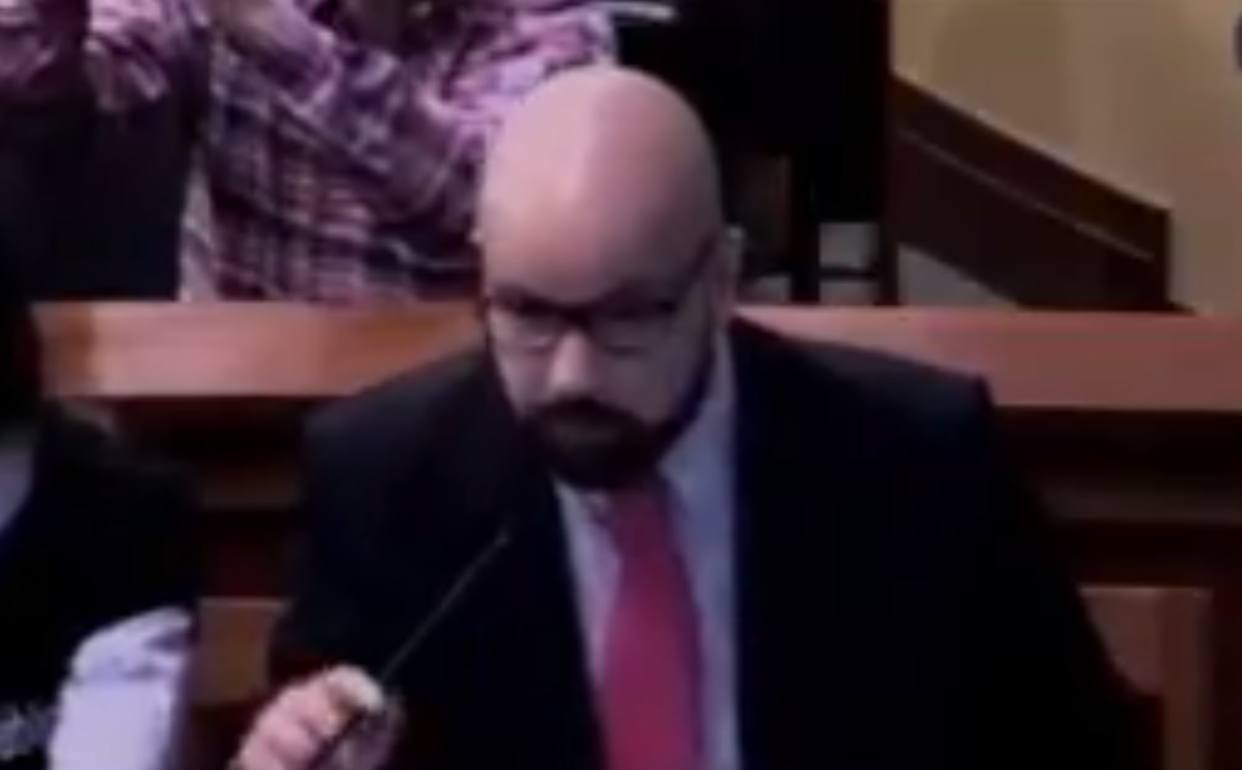
\includegraphics[width=300px]{100.jpg}%
\newline%
%
Eduardo Trujillo, representante del Centro de Derechos Humanos de la Universidad Católica Andrés Bello, señaló ante la Comisión Interamericana de Derechos Humanos que los migrantes y refugiados venezolano están expuestos a trata de personas y xenofobia.%
\newline%
%
“Hemos identificado las vulnerabilidades y riesgos específicos que acompañan a las personas migrantes y refugiadas provenientes de Venezuela en todas las etapas del desplazamiento”, indicó Trujillo.%
\newline%
%
El abogado resaltó que entre las vulnerabilidades y riesgos está la posibilidad de que puedan ser víctimas de trata de personas, xenofobia, violaciones al derecho a la vida y apatridia.%
\newline%
%
El representante del CDH de la UCAB señaló que la población venezolana migrante y refugiada se ha enfrentado y continúa enfrentándose a violaciones de derechos humanos.%
\newline%
%
“Hemos hecho énfasis en los grupos poblacionales de migrantes y refugiados en los que convergen múltiples factores de discriminación como género, raza, orientación sexual, entre otros que de forma intersesional aumentan los niveles de vulnerabilidad y afectan el goce y ejercicio de los derechos humanos de estos sectores de la población”, afirmó.%
\newline%
%
\end{document}